\documentclass[10pt]{article}

%------------------------------------------------------
%   PACKAGES
%------------------------------------------------------

% Default 
\usepackage{graphicx}
\usepackage[backend=biber,style=numeric,sorting=none]{biblatex}

% Additional
\usepackage{amsmath}
\usepackage{textcomp, gensymb}
\usepackage{placeins}
\usepackage{tabularray} 
\usepackage{xcolor}
\usepackage{placeins}
\usepackage{todonotes}
\newcommand{\td}[1]{\todo[linecolor=blue, backgroundcolor=blue!25,bordercolor=blue, size=\small]{#1}}

\addbibresource{references.bib}

\title{Microwave Optics I} 
\author{Rahmanyaz Annyyev, Hikmat Gulaliyev} 
\date{17 March 2024} 

\begin{document}

\maketitle

\begin{abstract}



\end{abstract}

\section{Introduction}

The electromagnetic spectrum is the range of all possible frequencies of electromagnetic radiation. The spectrum is divided into several regions, in order of decreasing frequency and increasing wavelength: gamma rays, X-rays, ultraviolet, visible light, infrared, microwaves, and radio waves. The microwave region of the electromagnetic spectrum is usually defined as being the range of frequencies from 1 GHz to 100 GHz. The wavelengths of microwaves are usually measured in centimeters. Microwaves are widely used in modern technology, for example in telecommunications, radar, and microwave ovens.

In this experiment, we will study the properties of microwaves and the behavior of microwave components. Since microwaves are invisible to the human eye, we will use a microwave transmitter and receiver to detect and measure the properties of microwaves. 

In part A of the experiment, we will measure the wavelength of microwaves using a microwave transmitter and receiver. The setup is shown in Figure \ref{fig:1}. The transmitter emits microwaves, which are then detected by the receiver. The receiver is mounted on a rail, and can be moved along the rail. The distance between the transmitter and receiver can be adjusted.

\begin{figure}[ht]
  \centering
  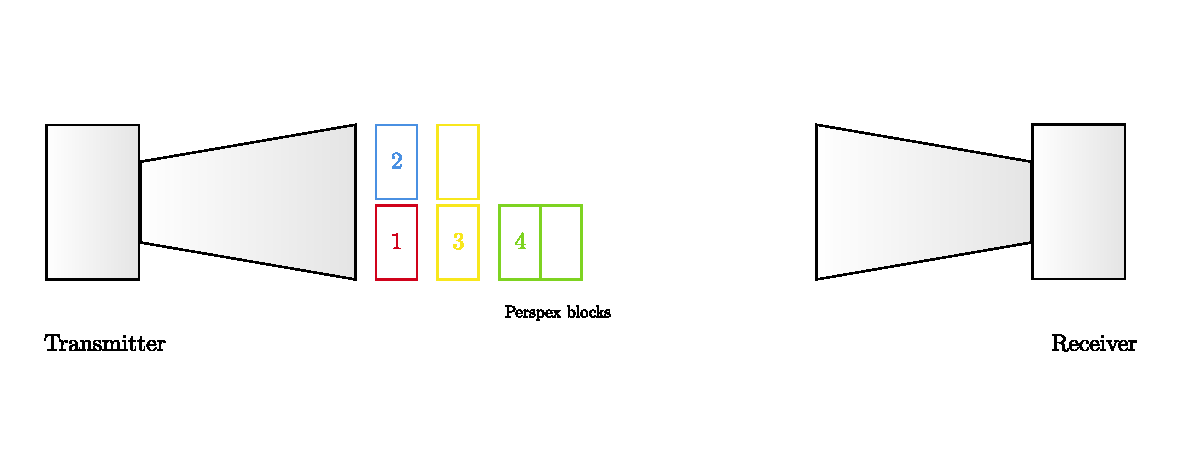
\includegraphics[scale=0.6]{figures/f1.pdf}
  \caption{Experimental setup for part B.}
  \label{fig:1}
\end{figure}

\section{Data \& Results}

\section{Discussion \& Conclusion}

\printbibliography

\end{document}